\chapter{Related Work}

\section{Pre-training Language Models in Machine Translation}

\cite{weng2020acquiring} In this paper, to address this appealing challenge, we design an A PT framework for acquiring the knowledge from pre-trained models to NMT. Specifically, our A PT framework has two modules. First, we propose a dynamic fusion mechanism which can learn a task-specific representation by adapting the general representation from pre-trained models, and adopt two controlling methods based on different granularities to fuse the task-specific representation into NMT dynamically. This method could provide rich contextual information for NMT to model sentence better. Second, we introduce a knowledge distillation paradigm to distill the knowledge from pre-trained models to NMT continuously. With this method, NMT could learn the knowledge about how to translate sources sentence to target sentences from parallel data and how to generate a better target sentence from monolingual data in the training process. Furthermore, according to our analysis and empirical results, we conclude that the best strategy for using the two methods in the encoder-decoder framework to improve translation quality.

\begin{figure}[h]
    {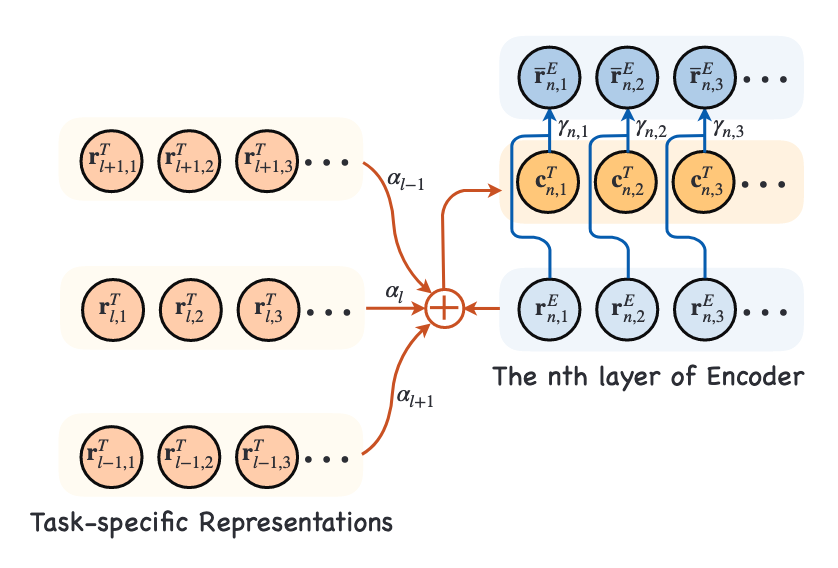
\includegraphics[width=0.95\textwidth]{img/dynamic_fusion.png}}
    \centering
    \caption{Illustration of seq2seq architecture. Figure reprinted from \cite{weng2020acquiring}.}
    \label{img:dyn_fn}
\end{figure}

\cite{yang2020towards}

compared to other tasks working well with direct BERT finetuning, NMT has two distinct characteristics, the availability of large training data (10 million or larger) and the high capacity of baseline NMT models (i.e. Transformer). These two characteristics require a huge number of updating steps during training in order to fit the high-capacity model well on massive data 1 . Updating too much leads to the catastrophic forgetting problem (Goodfellow et al. 2013), namely too much updating in training make the BERT forget its universal knowledge from pre-training. The assumption lies well with previous observations that fixed BERT improves NMT a bit and fine-tuning BERT even offers no gains. In this paper, we propose the concerted training approach (CT NMT ). Specifically, we introduce three techniques to integrate the power of pre-trained BERT and vanilla NMT, namely asymptotic distillation, dynamic switch for knowledge fusion, and ratescheduled updating. First, an asymptotic distillation (AD) technique is introduced to keep remind the NMT model of BERT knowledge. The pre-trained BERT serves as a teacher network while the encoder of the NMT model serves as a student. The objective is to mimic the original teacher network by minimizing the loss (typically L2 or cross-entropy loss) between the student and the teacher in an asymptotic way. The asymptotic distillation does not introduce additional parameters therefore it can be trained efficiently. Secondly, a dynamic switching gate (DS) is introduced to combine the encoded embedding from BERT and the encoder of NMT. Based on the source input sentence, it provides an adaptive way to fuse the power of BERT and NMT's encoder-decoder network. The intuition is that for some source sentences BERT might produce a better encoded information than NMT's encoder while it is opposite for other sentences. Thirdly, we develop a scheduling policy to adjust the learning rate during the training. Without such a technique, traditionally BERT and NMT are updated uniformly.  However, a separate and different updating pace for BERT LM is beneficial for the final combined model. Our proposed rate-scheduled learning effectively controls the separate paces of updating BERT and NMT networks according to a policy. With all these techniques combined, CT NMT empirically works effectively in machine translation tasks.

\begin{figure}[h]
    {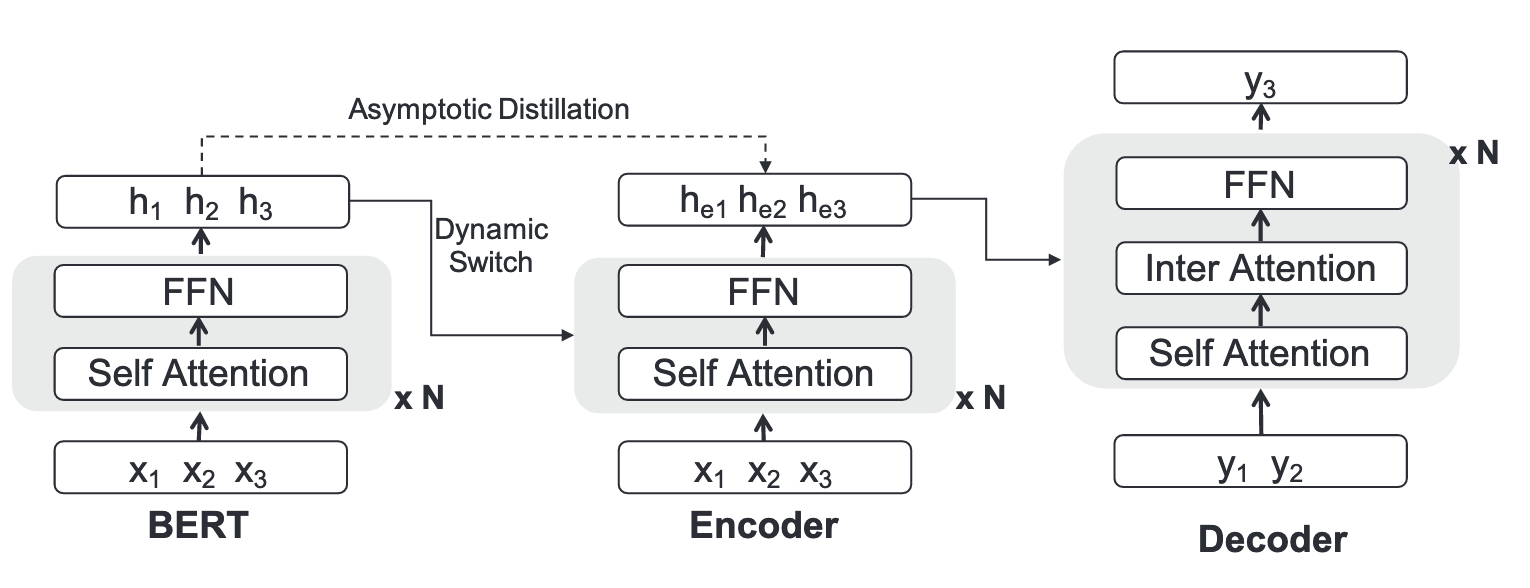
\includegraphics[width=0.95\textwidth]{img/ctnmt.png}}
    \centering
    \caption{Illustration of seq2seq architecture. Figure reprinted from \cite{yang2020towards}.}
    \label{img:ctnmt}
\end{figure}

Intuitively, as BERT is learned with a generative objective via Masked Language Modeling (MLM) during the pre-training stage, a natural assumption is that this training objective should have learned essential, bidirectional, contextual knowledge that can help enhance text generation. Unfortunately, this MLM objective is not auto-regressive, which encumbers its direct application to auto-regressive text generation in practice. In this paper, we tackle this challenge by proposing a novel and generalizable approach to distilling knowledge learned in BERT for text generation tasks. We first propose a new Conditional Masked Language Modeling (C-MLM) task, inspired by MLM but requiring additional conditional input, which enables fine-tuning pre-trained BERT on a target dataset. In order to extract knowledge from the fine-tuned BERT and apply it to a text generation model, we leverage the fine-tuned BERT as a teacher model that generates sequences of word probability logits for the training samples, and treat the text generation model as a student network, which can effectively learn from the teacher's outputs for imitation. The proposed approach improves text generation by providing a good estimation on the word probability distribution for each token in a sentence, consuming both the left and the right context, the exploitation of which encourages conventional text generation models to plan ahead. With our proposed approach, BERT's looking into the future ability can act as an effective regularization method, capturing subtle long-term dependencies that ensure global coherence and in consequence boost model performance on text generation.

\cite{chen2019distilling}

\begin{figure}[h]
    {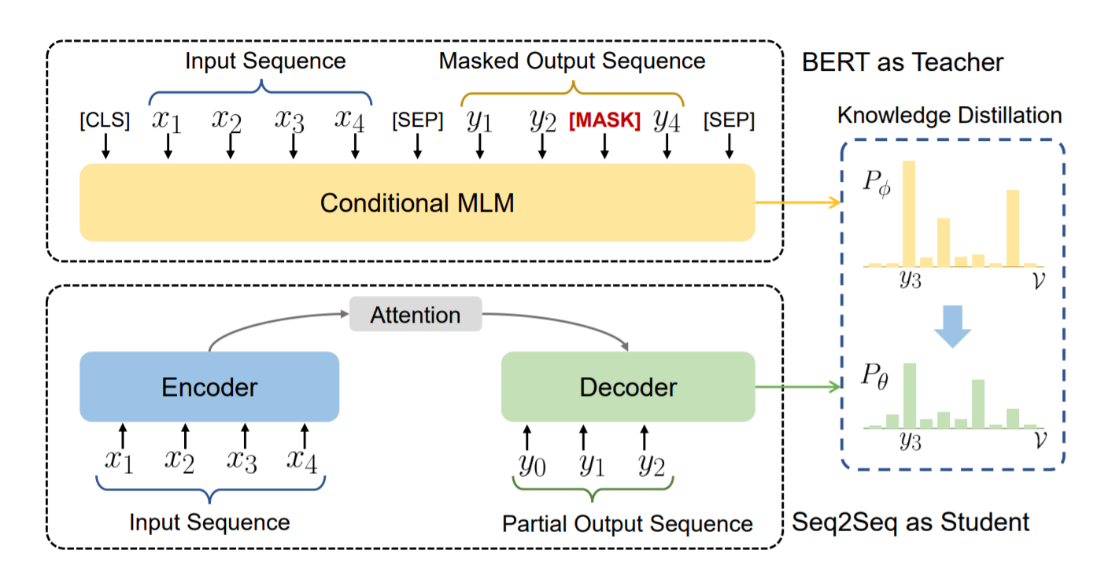
\includegraphics[width=0.95\textwidth]{img/bert_distill.png}}
    \centering
    \caption{Illustration of seq2seq architecture. Figure reprinted from \cite{chen2019distilling}.}
    \label{img:bert_distill}
\end{figure}

\section{Adapters in Sequence-to-Sequence}
Works on incorporating adapters in machine translation
\subsection{Adapters in NLU and Automatic Speech Recognition}
\subsection{Adapters in Machine Translation}
\subsection{Placement of Adapters}
% \section{Fine-tuning in Sequence-to-Sequence Framework}